\documentclass[letterpaper,12pt]{article}
\usepackage{graphicx}	
\usepackage{natbib}	
\usepackage{amsmath}	
\usepackage{bbm}	%
\usepackage[left=3cm,top=3cm,right=3cm]{geometry}

\renewcommand{\topfraction}{0.85} \renewcommand{\textfraction}{0.1} 
\parindent=0cm

\newcommand{\nyu}{$^1$}
\newcommand{\mpia}{$^2$}
\newcommand{\sdss}{{\it SDSS}}

\usepackage{url}

\title{A Mixture of Gaussians / Factor Analyzers Model for the Sloan Digital Sky Survey}
\author{Ross Fadely\nyu, Daniel Foreman-Mackey\nyu, Rob Fergus\nyu, \\ 
David W. Hogg\nyu$^,$\mpia~,  et al. \\
\\
\small
\nyu Center for Cosmology and Particle Physics,
                        Department of Physics, New York University,\\ \small
                        4 Washington Place, New York, NY, 10003, USA \\
\small\mpia Max-Planck-Institut f\"ur Astronomie,
                        K\"onigstuhl 17, D-69117 Heidelberg, Germany \\
}
\begin{document}
\maketitle

\begin{abstract}
\end{abstract}

\section{Introduction}

\begin{itemize}


\item \sdss\, analysis at the pixel-level has (mostly) been restricted to 
a `catalog' approach, where a set of measurements are made using 
(often) fix heuristics and relatively little probabilistic information is returned.  
A natural extension to this approach is to build probabilistic catalogs (e.g., 
Tractor).

\item An alternative type of analysis is to probabilistically model the distribution 
of pixel values, disconnected from (almost) any knowledge of physics or the 
domain of the values.  

\item Motivate from a computer vision view.

\item Describe MOG and MOFA.

\item Describe what can be done.


\end{itemize}

\section{Technical Details}

\subsection{Patches}


We take $7\times7$ patches with single pixel steps across a given \sdss\, field.  
One of the effects is that each source is sampled many times as the patch 
window is moved across the image.  An important consequence of this is that 
the centroids of the pixel values in the patches are shifted around the pixel grid
(Figure \ref{fig:unflipped}), causing MOG and MOFA models to need to place a 
mixture component at each location around the pixel grid.  
\\ \\
Instead, if we take the images to be isotropic (not fully true for \sdss), we can 
view each patch as an arbitrary rotation of a given source.  That is, if we rotate 
patches to have centroids in similar locations, we can reduce the effective 
number of components needed to construct the model, as long as we view the 
rotation as a fair representation of the patch.  We rotate the patches such that 
the centroids lie in the region $45-90^{\,\circ}$ above the `x' axis of the patch, 
or in the NNW octile by analogy to astronomical definitions.  Figure 
\ref{fig:flipped} shows the rotated and/or flipped versions of patches seen in 
Figure \ref{fig:unflipped}.

\begin{figure}
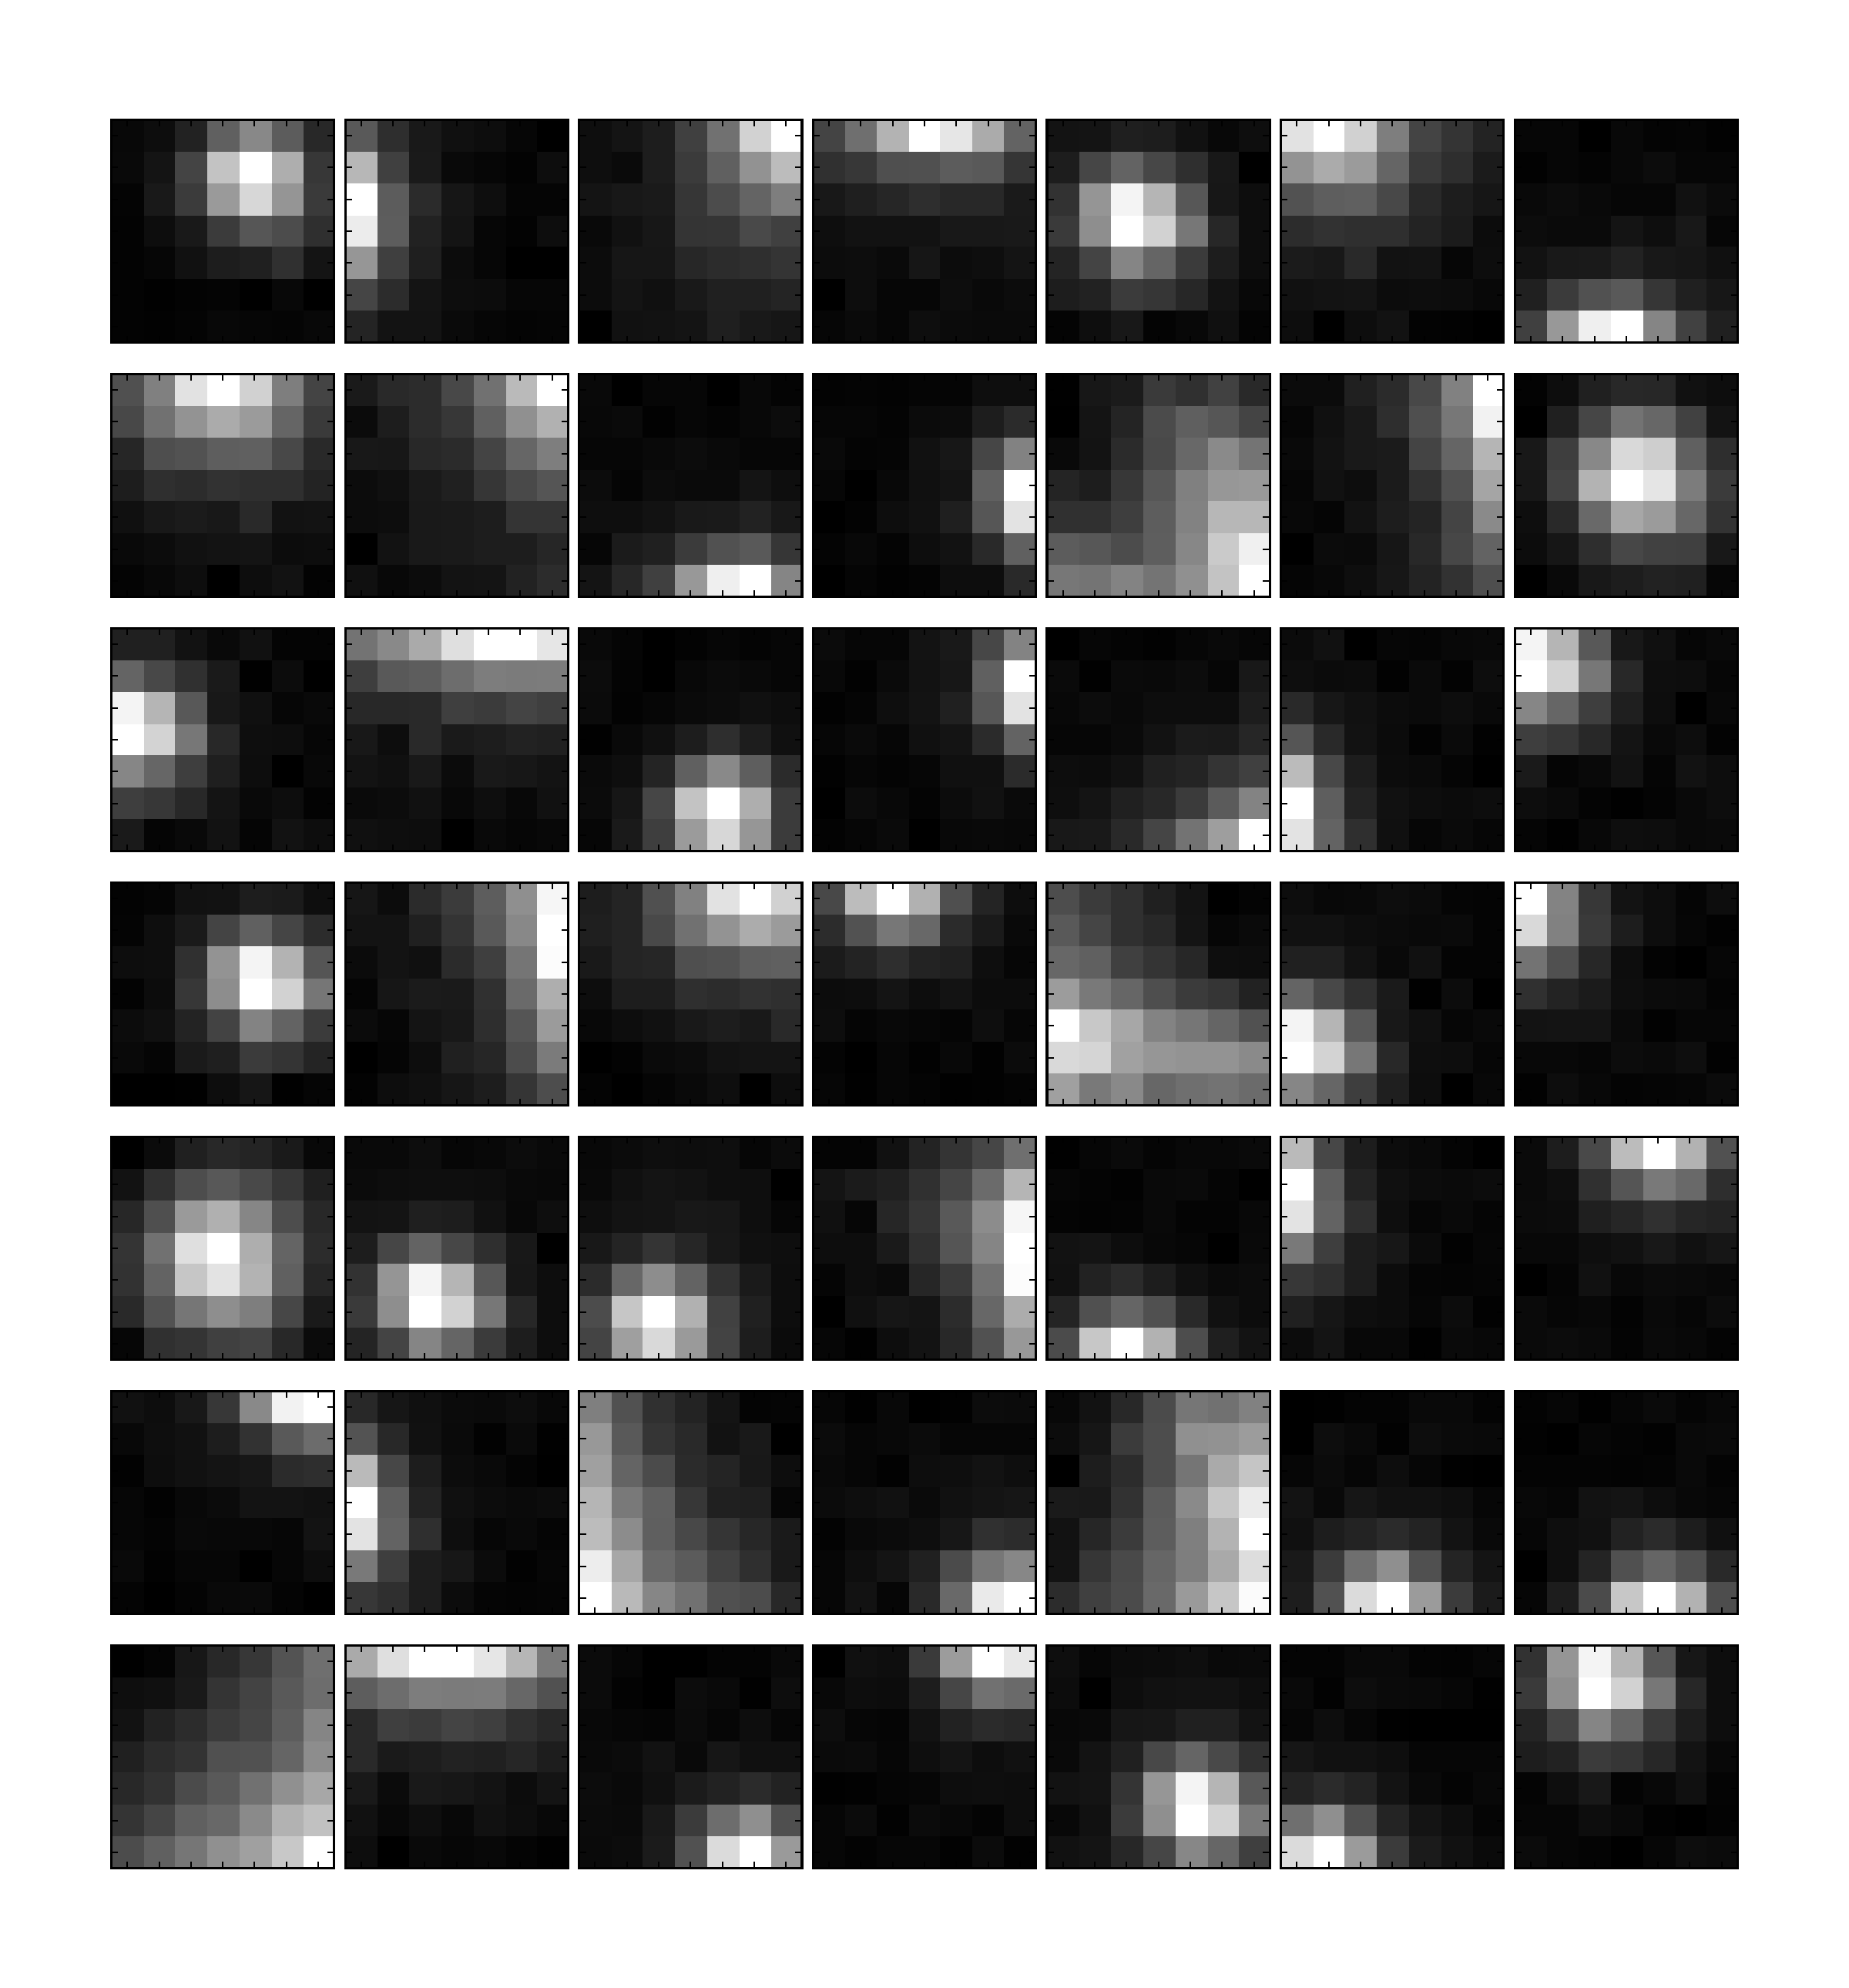
\includegraphics[clip=true, trim=0cm 0cm 0.0cm 0.cm,width=12cm]{figures/unflipped.pdf}
\caption{Patches taken from \sdss\, data with a stride of one pixel.  Note how 
the patches contain repeated sources, whose centroids move around in 
patch location.}
\label{fig:unflipped}
\end{figure}

\begin{figure}
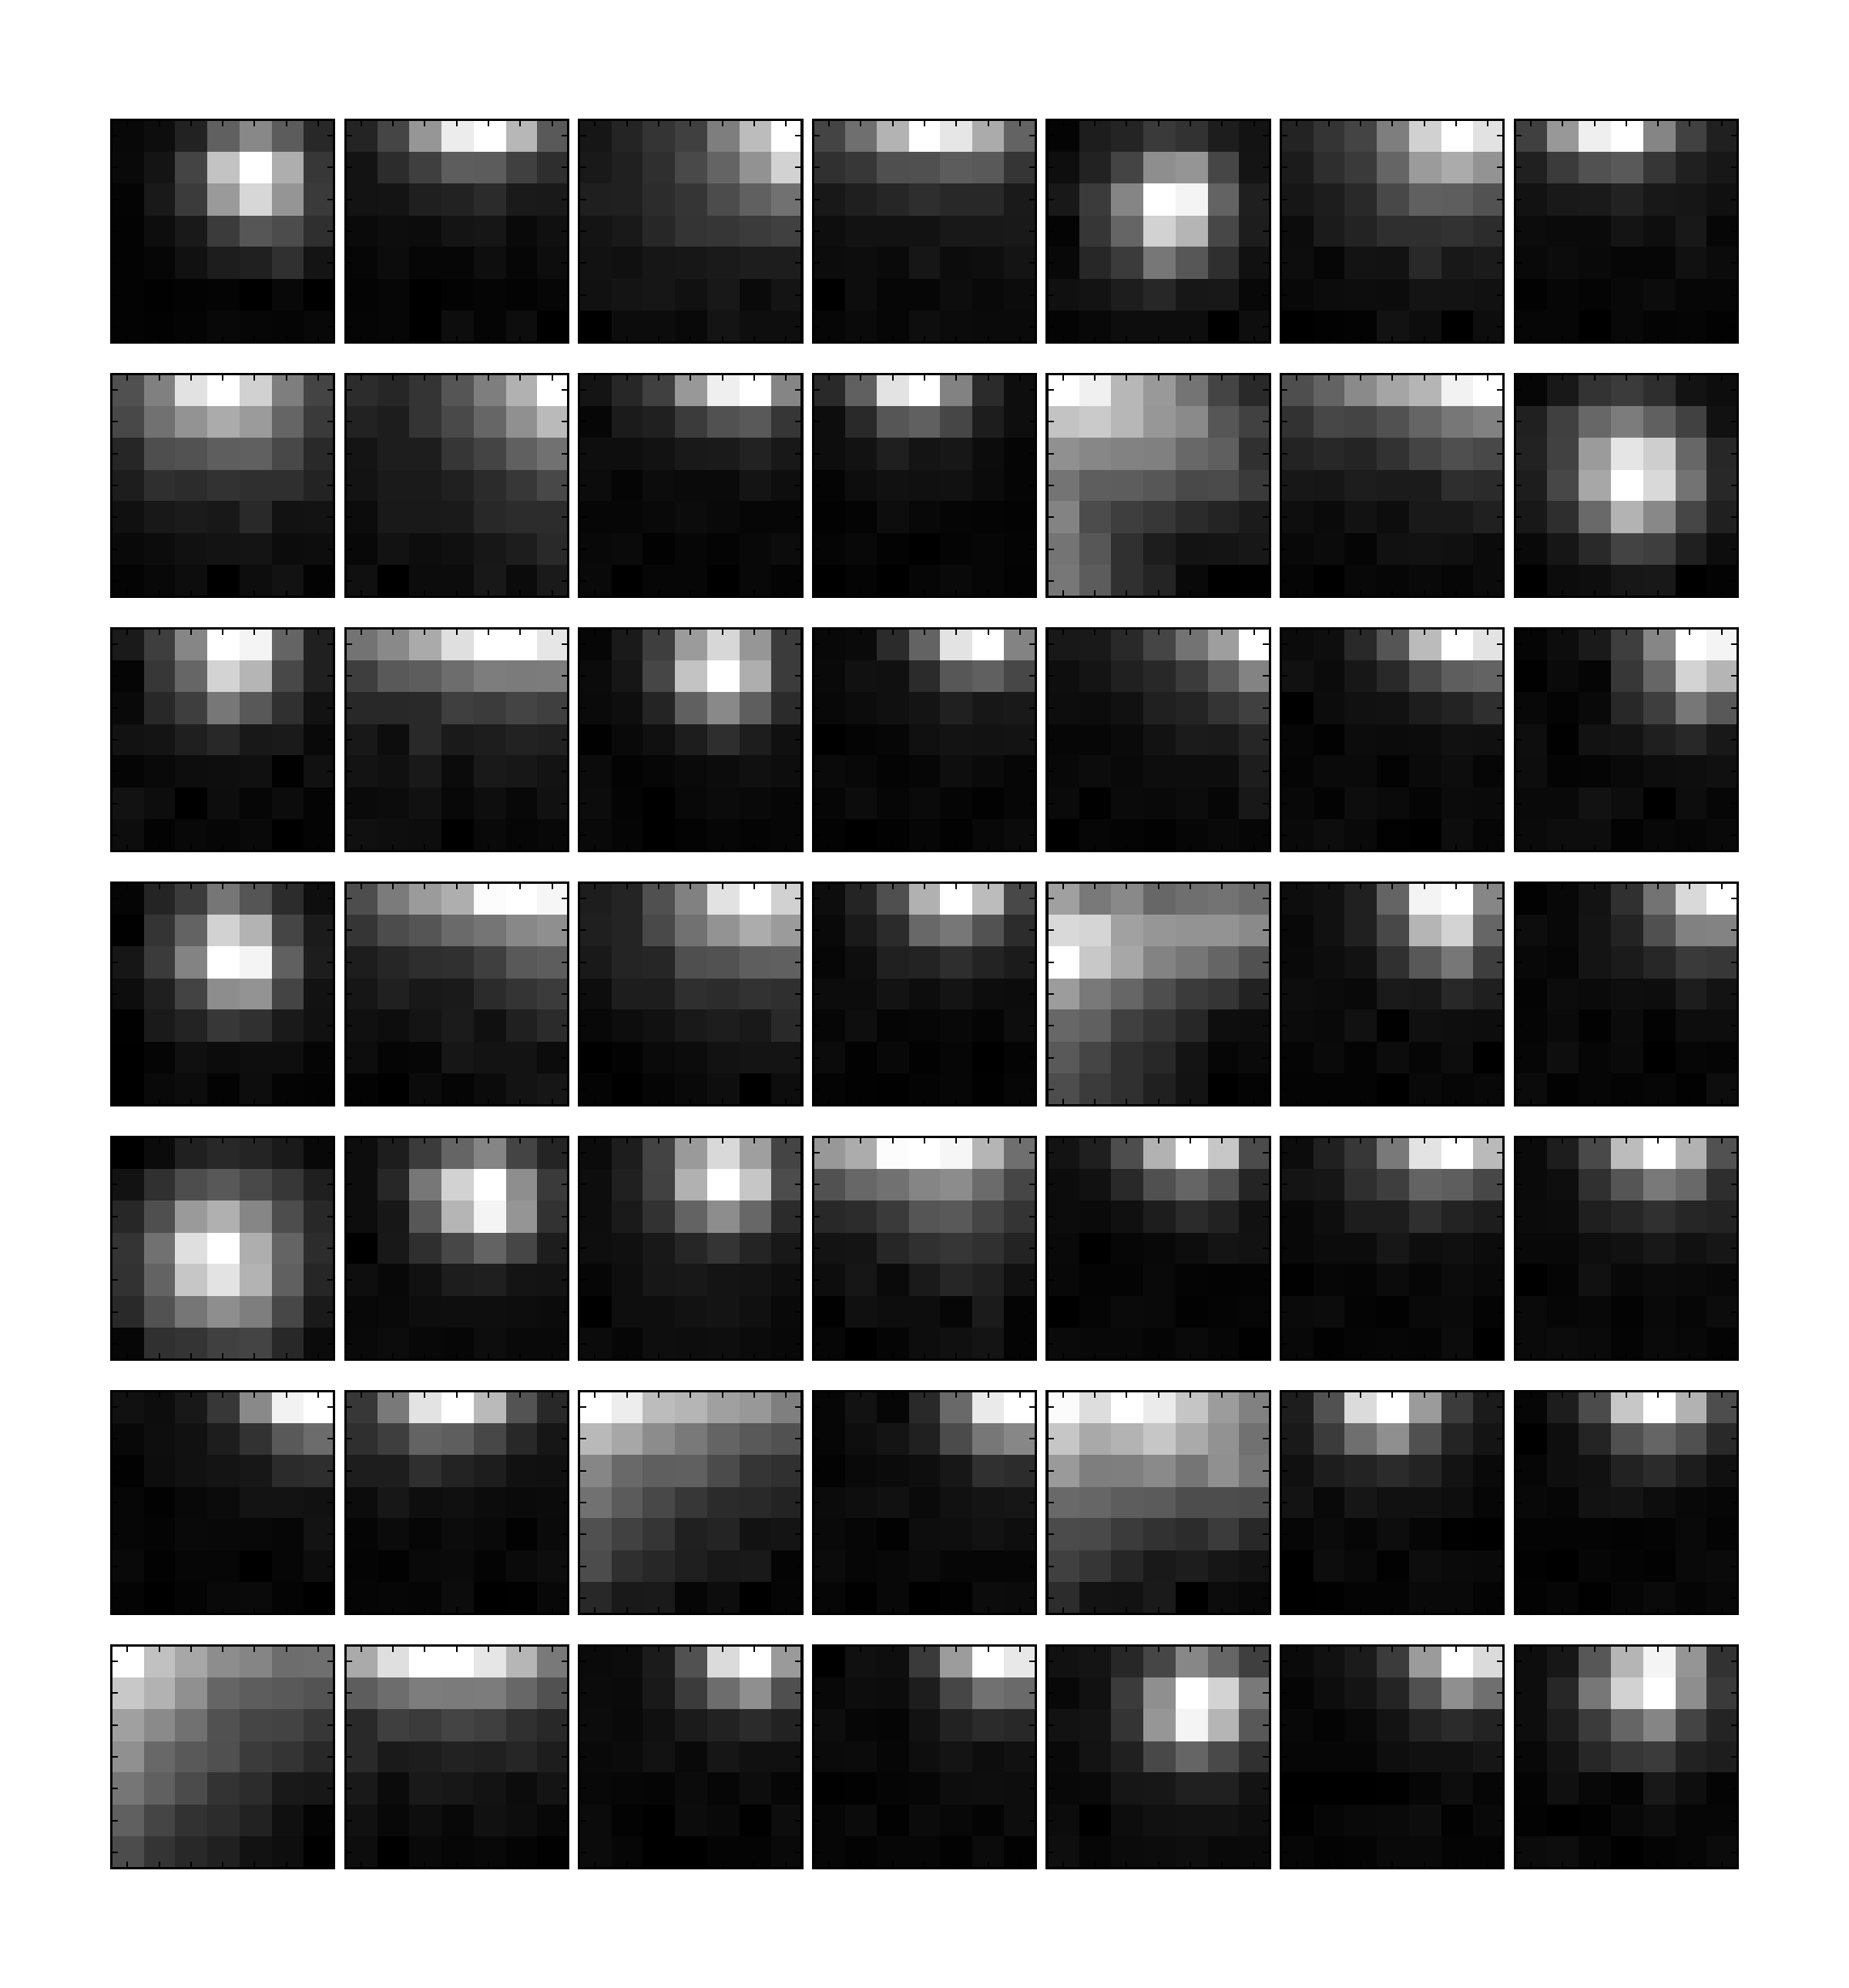
\includegraphics[clip=true, trim=0cm 0cm 0.0cm 0.cm,width=12cm]{figures/flipped.pdf}
\caption{Patches from Figure \ref{fig:unflipped}, but rotated and flipped to 
have their centroids in a similar location.  Doing so reduces the number 
of mixture components needed to explain the data.}
\label{fig:flipped}
\end{figure}

\end{document}


